% Converted from the reference-locked manuscript.
% Final display and interpretation pass; mathematical definitions remain source-verified.
\section*{Results}

\subsection*{Mouse dataset integration and the Walesky injury--recovery reference}

We developed TrajRisk to model hepatocyte state progression during acetaminophen (APAP)-induced liver injury by combining trajectory inference, learned transition probabilities, and graph neural network propagation into a unified framework (\FigRef{1}{A}).

To capture complementary phases of injury and recovery, we assembled four publicly available mouse single-cell RNA-sequencing datasets. The Walesky dataset served as the primary reference cohort, containing hepatocytes sampled across the canonical APAP time course (0~h, 6~h, 24~h, 48~h, and 96~h) (n = 6,582 hepatocytes after timepoint selection and exclusion of partial hepatectomy samples), while three additional datasets provided independent cohorts spanning early injury, recovery, and persistent compensation: the Umbaugh 2~h dataset (n = 21,409), the Ben-Moshe dataset (n = 2,770), and the Umbaugh 48~h/72~h dataset (n = 5,306) (\FigRef{1}{B}). Quality-control characteristics of the three external mouse cohorts are summarized in \FigRefs{S1}{A--S1C}. Together these datasets comprised 36,067 hepatocytes spanning multiple platforms, laboratories, and injury/recovery phases.

Following integration with scVI (\hyperref[sec:methods]{Methods}), all four mouse datasets were represented in a shared 30-dimensional latent space (\FigRef{1}{C}). Dataset average silhouette width (ASW) was low (0.039), consistent with intermixing, although residual cross-platform structure motivated restriction of trajectory inference to Walesky hepatocytes. Treatment and sampling-time overlays showed heterogeneous injury- and recovery-associated states. These descriptive diagnostics assess the representation used for subsequent analyses; low dataset ASW alone does not establish preservation of every biological distinction.

Trajectory inference on the Walesky cohort using Monocle 3\cite{ref047} reconstructed a continuous progression from healthy hepatocytes toward injury-associated states, diverging into recovery and persistent-compensation trajectories (\FigRef{1}{D}). Pseudotime correlated significantly with experimental time (Spearman \ensuremath{\rho} = 0.5051, p < 2.2\ensuremath{\times}10\textsuperscript{-16}), while remaining non-linear enough to capture heterogeneous recovery responses. 6~h hepatocytes occupied the highest pseudotime values relative to the control root, consistent with peak acute injury, while later timepoints showed increasing heterogeneity as hepatocytes returned toward homeostasis or remained in persistent compensation (\FigRef{2}{A}). Raw Monocle pseudotime distributions within each sampling timepoint are shown in \FigRef{S2}{A}.

The integrated representation and Walesky-restricted pseudotime provided the features and reference states used to construct directed temporal graphs.

\begin{figure*}[!tp]
\centering
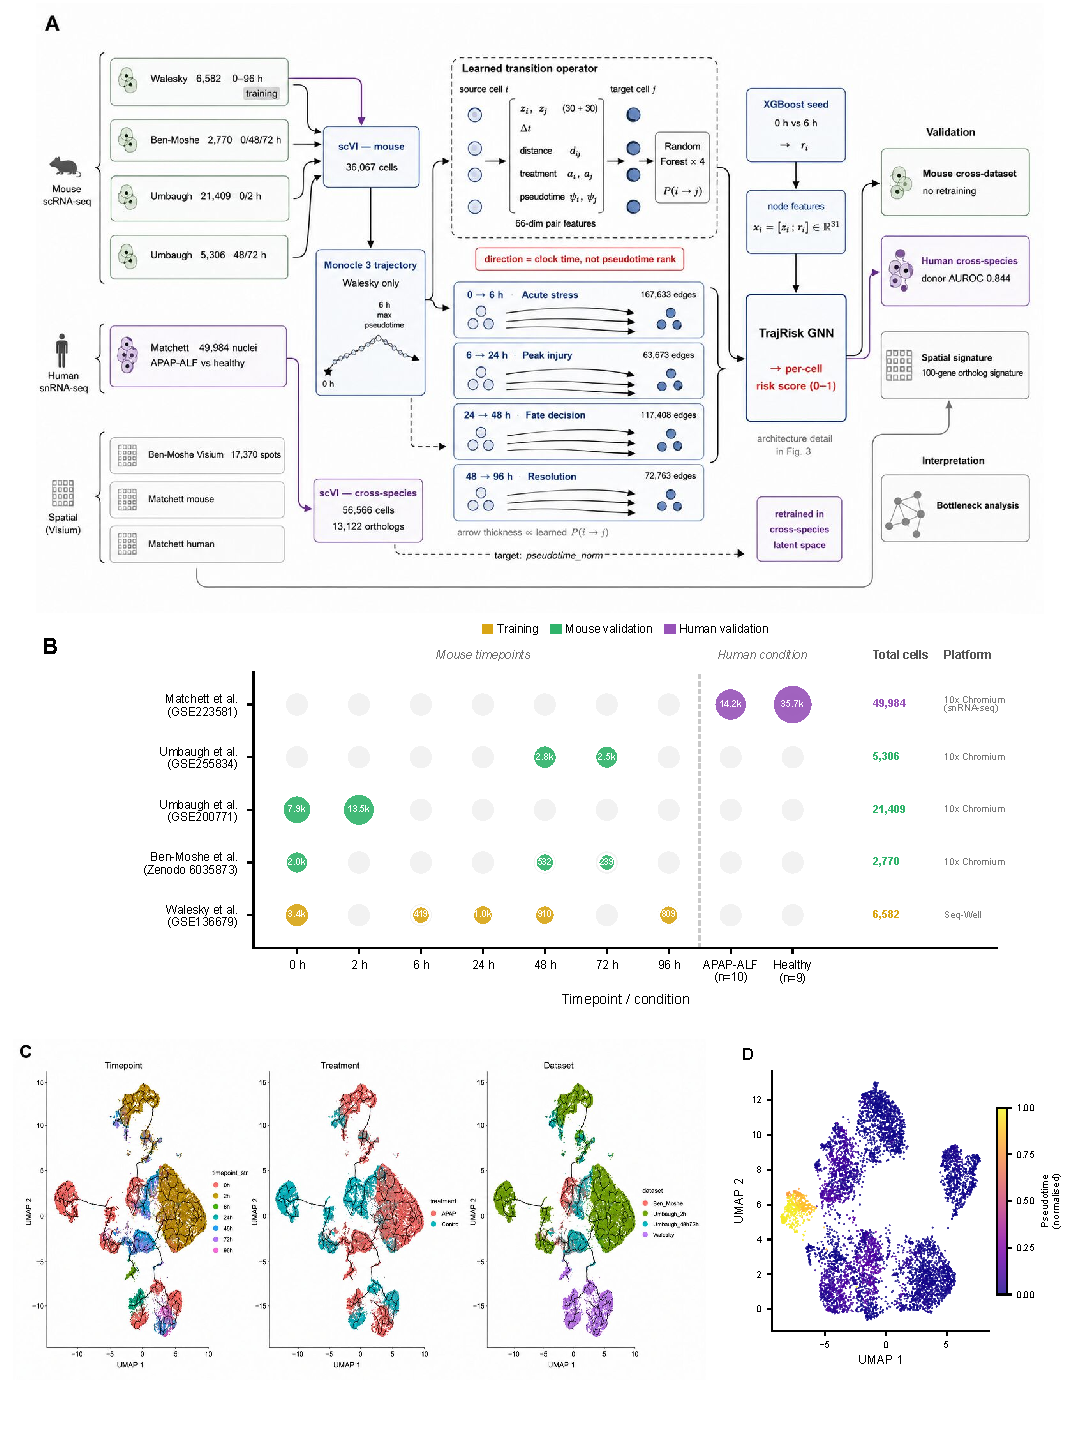
\includegraphics[width=\textwidth,trim={0.000bp 395.000bp 0.000bp 0.000bp},clip]{figures/figure_1.pdf}
\caption{\textbf{\FigOneTitle{}} \textbf{(A)} \FigOneA{}}
\label{fig:1}
\end{figure*}
\begin{figure*}[!tp]
\centering
\ContinuedFloat
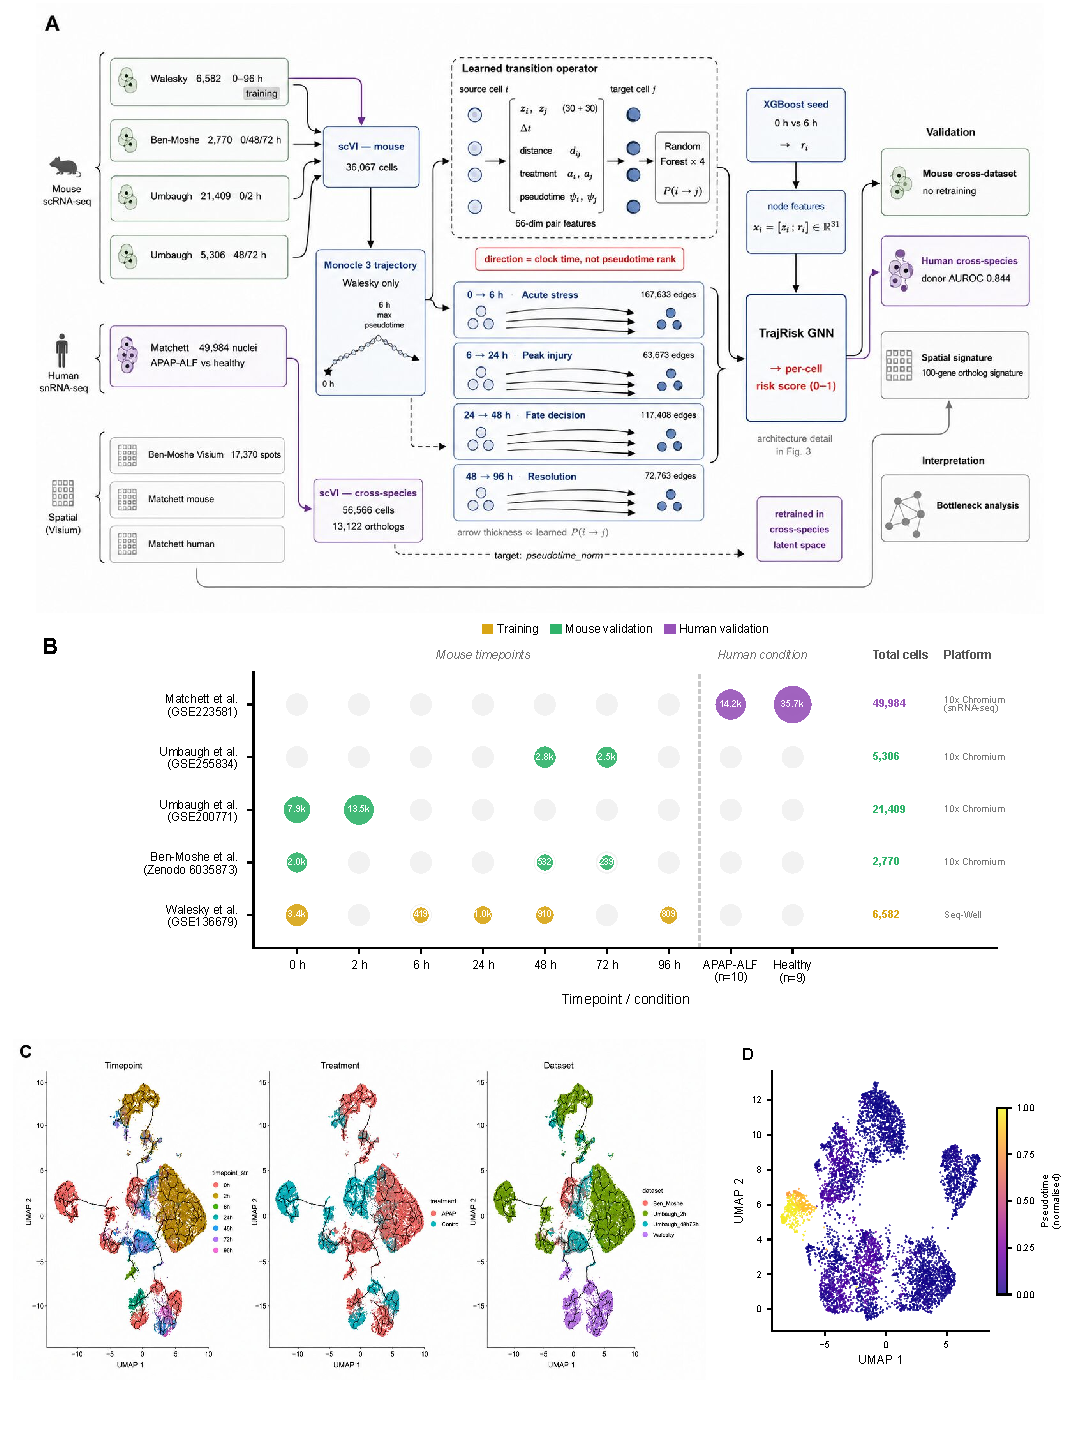
\includegraphics[width=\textwidth,trim={0.000bp 192.000bp 0.000bp 299.000bp},clip]{figures/figure_1.pdf}
\par\vspace{8pt}
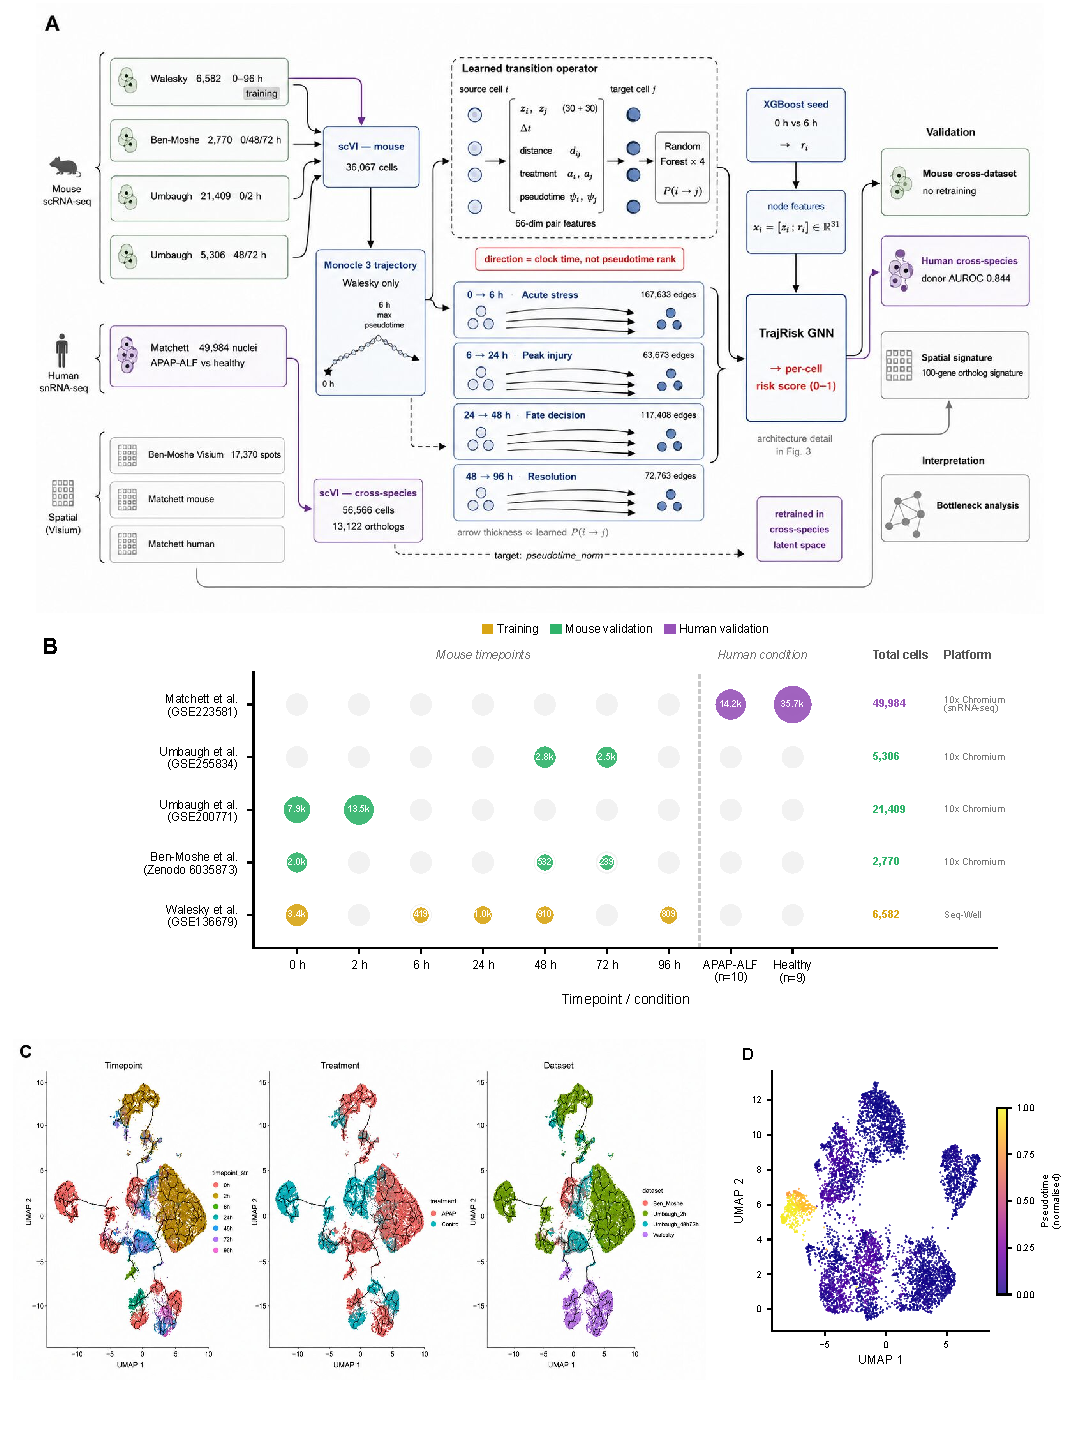
\includegraphics[width=\textwidth,trim={0.000bp 4.000bp 0.000bp 502.000bp},clip]{figures/figure_1.pdf}
\caption{\textbf{\FigOneTitle{} (continued)} \textbf{(B)} \FigOneB{} \textbf{(C)} \FigOneC{} \textbf{(D)} \FigOneD{} \FigOneNotes{}}
\end{figure*}

\subsection*{Random Forest classifiers learn directed, treatment-aware transition probabilities}

We trained one Random Forest classifier per temporal scale to predict nearest-neighbor-defined cell-pair transition labels (\hyperref[sec:methods]{Methods}). Five-fold stratified cross-validation yielded AUROC values of 0.9936 \ensuremath{\pm} 0.0002 (Scale 1, 0~h \ensuremath{\rightarrow} 6~h), 0.9871 \ensuremath{\pm} 0.0011 (Scale 2, 6~h \ensuremath{\rightarrow} 24~h), 0.9901 \ensuremath{\pm} 0.0004 (Scale 3, 24~h \ensuremath{\rightarrow} 48~h), and 0.9929 \ensuremath{\pm} 0.0009 (Scale 4, 48~h \ensuremath{\rightarrow} 96~h), with out-of-bag accuracy estimates of 0.961, 0.949, 0.955, and 0.965, respectively (\FigRef{2}{B}; \TableRef{S1}). The most important single feature across all scales was Euclidean distance in scVI latent space, consistent with the k-nearest-neighbor-based training labels. The learned transition matrices diverged substantially from a distance-only Gaussian kernel (\FigRef{2}{C}): row-wise Pearson correlations between each learned matrix and its Gaussian baseline were low (Scale 1: 0.246; Scale 2: 0.187; Scale 3: 0.249; Scale 4: 0.403), showing that the learned weights differ from a distance-only kernel. The RF classifiers also receive treatment, normalized pseudotime, and latent coordinates. Their cross-validation evaluates agreement with the constructed neighbor labels rather than independently observed biological transitions.

The resulting matrices remained numerically close to the stochasticity constraint after sparsification (row sums = 1.000, SD < 10\textsuperscript{-6}) and retained high sparsity (99.6-99.9\%). Per-cell transition entropy varied across scales (\FigRef{2}{D}; \TableRef{S1}). Scale 2 had the highest mean entropy (4.88 \ensuremath{\pm} 0.42 nats), and Scale 1 the lowest (3.81 \ensuremath{\pm} 0.26 nats); Scales 3 and 4 had intermediate means of 4.58 and 4.24 nats. These values summarize heterogeneity in outgoing transition weights, rather than the number or probability of biological fates available to a cell.

\begin{figure*}[!tp]
\centering
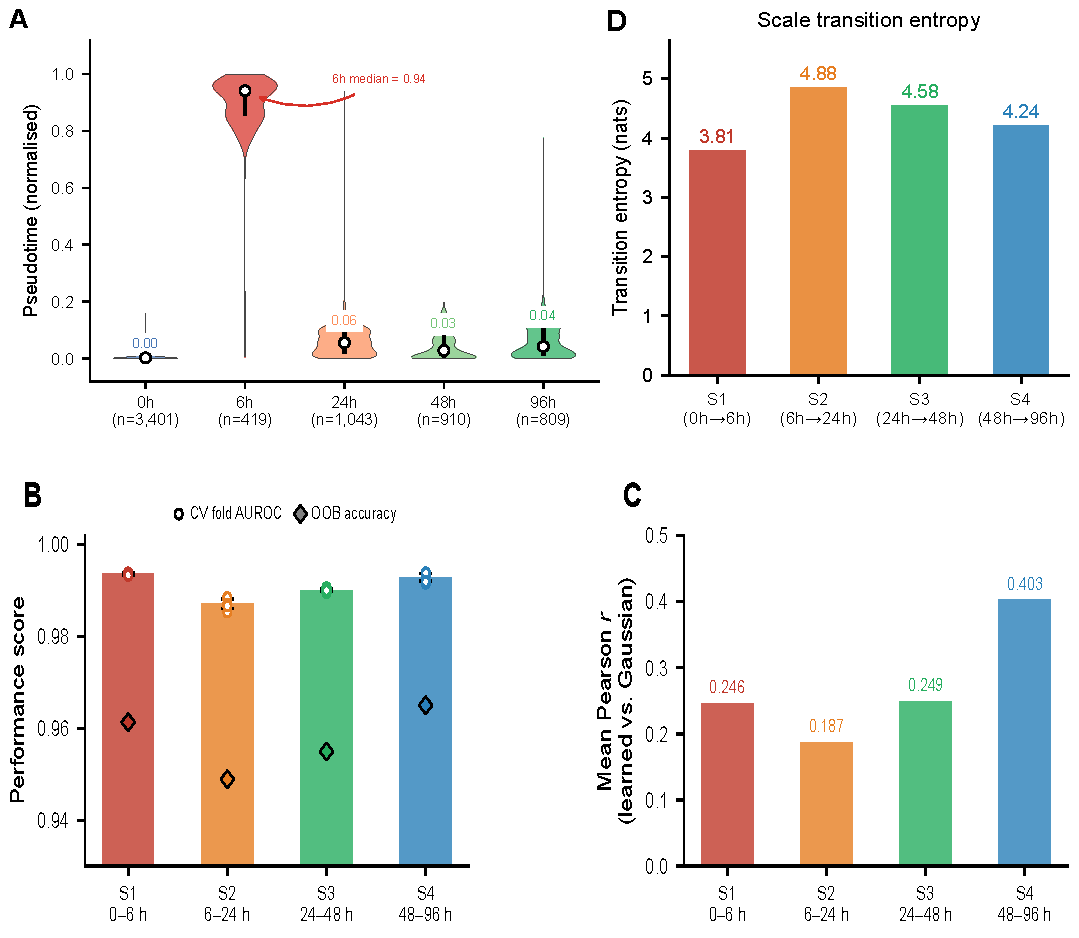
\includegraphics[width=\textwidth,trim={0.000bp 0.000bp 0.000bp 0.000bp},clip]{figures/figure_2.pdf}
\caption{\textbf{\FigTwoTitle{}} \textbf{(A)} \FigTwoA{} \textbf{(B)} \FigTwoB{} \textbf{(C)} \FigTwoC{} \textbf{(D)} \FigTwoD{} \FigTwoNotes{}}
\label{fig:2}
\end{figure*}

\subsection*{TrajRiskGNN learns biologically coherent trajectory-state representations}

The TrajRiskGNN architecture is summarized in \FigRef{3}{A}. The validation-AUROC-best checkpoint at epoch 144 was used for downstream analyses; training history and validation performance are shown in \FigRefs{3}{B--3D}. The model achieved a validation AUROC of 0.9071 (95\% CI 0.8843--0.9310), AUPRC of 0.7707, and a Spearman correlation of 0.5814 with normalized pseudotime (p = 4.65\ensuremath{\times}10\textsuperscript{-120}; \TableRef{S2A}). The train-validation Spearman gap was 0.029.

TrajRisk scores followed a pattern consistent with the reference injury trajectory (\FigRef{3}{E}). 0~h root hepatocytes had the lowest mean score (0.008; 0.0\% exceeding a predicted-score threshold of 0.10), while 6~h APAP hepatocytes, sampled during acute injury, had the highest mean score (0.917; 99.3\% exceeding threshold). Mean scores declined at 24~h (0.047, 5.2\% exceeding) and 48~h (0.030, 0.9\%), with a modest rise at 96~h (0.045, 5.6\%) consistent with a persistent compensation subpopulation. Scale-association analysis showed that Scale 1 (Acute Stress) embedding norms were positively associated with the TrajRisk score, whereas Scale 3 (Fate Decision) embedding norms were negatively associated with it (Spearman \ensuremath{\rho} = +0.325 and -0.372, respectively; \FigRef{3}{F}). A PCA of the concatenated 256-dimensional multi-scale representation, colored by sampling timepoint and by predicted TrajRisk score, is shown in \FigRefs{S2}{B and S2C}.

\begin{figure*}[!tp]
\centering
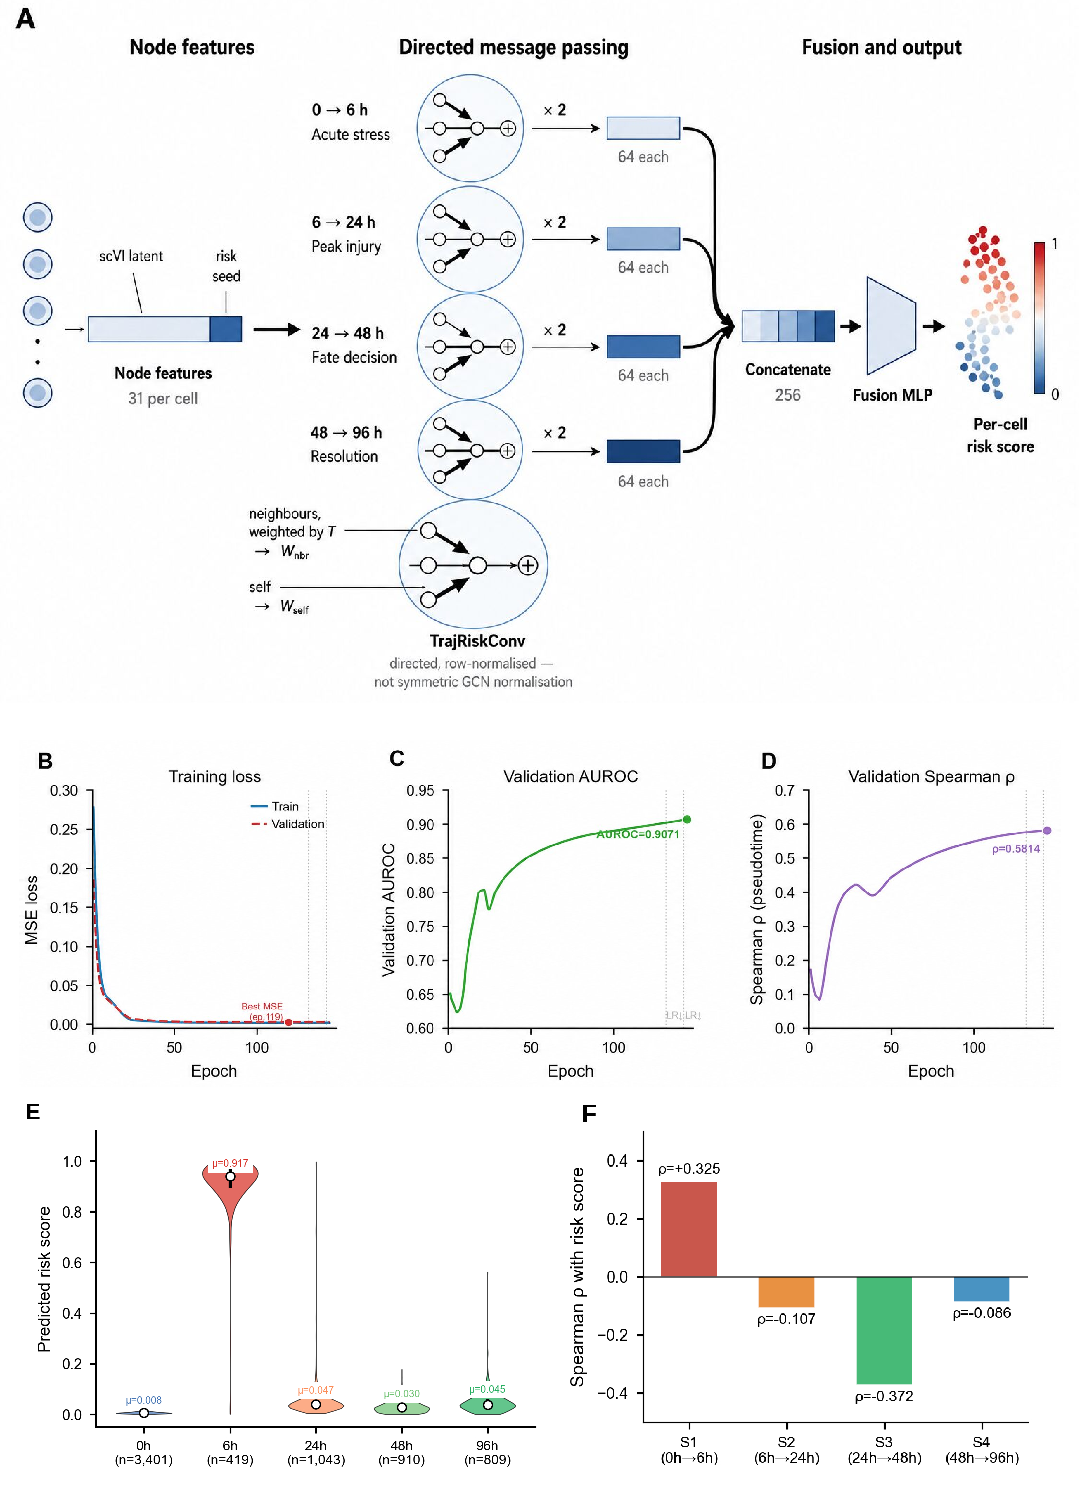
\includegraphics[width=\textwidth,trim={0.000bp 372.000bp 0.000bp 0.000bp},clip]{figures/figure_3.pdf}
\caption{\textbf{\FigThreeTitle{}} \textbf{(A)} \FigThreeA{}}
\label{fig:3}
\end{figure*}
\begin{figure*}[!tp]
\centering
\ContinuedFloat
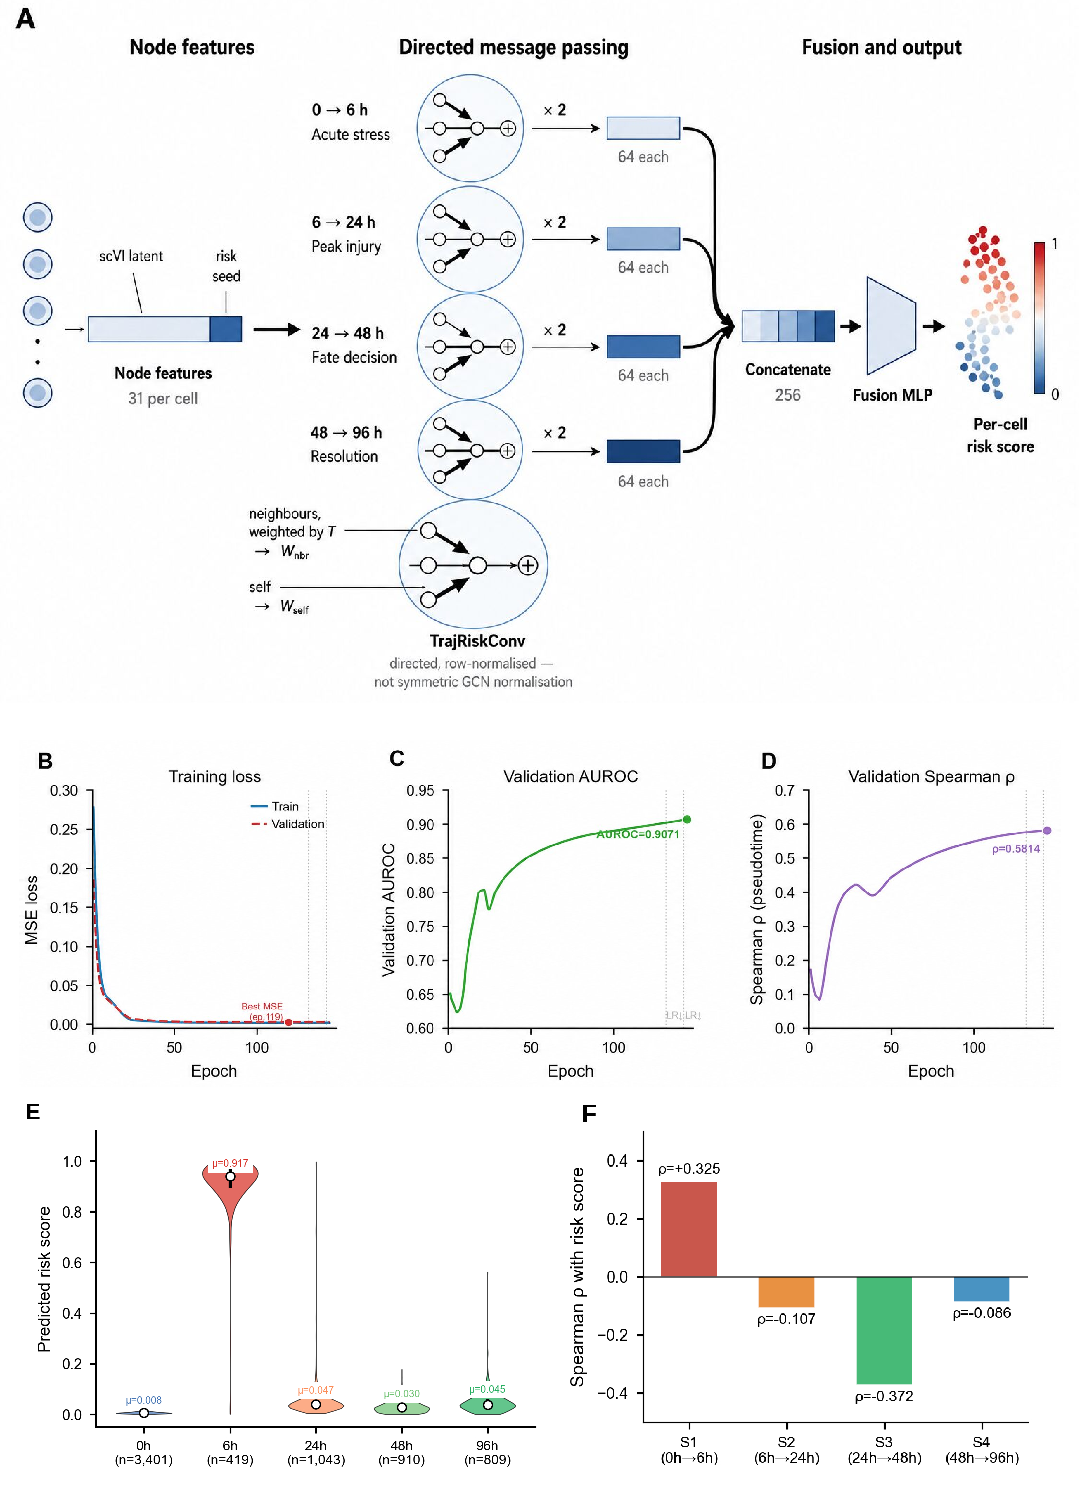
\includegraphics[width=\textwidth,trim={0.000bp 3.000bp 0.000bp 352.000bp},clip]{figures/figure_3.pdf}
\caption{\textbf{\FigThreeTitle{} (continued)} \textbf{(B)} \FigThreeB{} \textbf{(C)} \FigThreeC{} \textbf{(D)} \FigThreeD{} \textbf{(E)} \FigThreeE{} \textbf{(F)} \FigThreeF{} \FigThreeNotes{}}
\end{figure*}

\subsection*{Benchmark comparisons show timepoint-dependent performance}

We benchmarked TrajRisk against four baselines on the fixed 1,318-cell Walesky validation set (\FigRef{4}{A}; \TableRef{S2A}). Expression-only XGBoost\cite{ref048} regression (B1) achieved higher global AUROC than TrajRisk (0.9582 versus 0.9071). Both models use expression-derived features to predict expression-derived pseudotime. The TrajRisk graphs additionally incorporate reference pseudotime during construction, including for validation cells; this is a transductive within-reference evaluation rather than an independent test on unseen cells.

TrajRisk had higher global AUROC than Gaussian scalar propagation (0.856), the development-selected single-scale GNN (0.850), and expression distance from baseline controls (0.800), with one-sided paired-bootstrap p < 0.001 for each comparison (\FigRef{4}{A}). The initial XGBoost seed achieved AUROC 0.875, compared with 0.907 for TrajRisk. The seed is an acute-state classifier trained on 0~h versus 6~h cells, whereas B1 directly regresses continuous pseudotime; these are distinct expression-only comparators.

Reduced-model comparisons showed lower AUROC when learned RF transitions were replaced by Gaussian transitions (decrease of 8.1 percentage points), the seed was removed (7.9 points), one temporal scale was retained (5.7 points), or the complete GNN was replaced by scalar RF propagation (5.4 points) (\FigRefs{4}{A and 4B}; \TableRefs{S2A}{S2B}). These comparisons support sensitivity to model configuration but do not isolate every component: scalar RF propagation jointly removes nonlinear message aggregation and node-feature integration. The primary model was selected using validation AUROC, while GNN ablations used an inner development split, giving the primary model a checkpoint-selection advantage (\hyperref[sec:methods]{Methods}).

We also evaluated discrimination within recovery timepoints using average precision (AUPRC), with positive labels defined by normalized pseudotime > 0.10 (\FigRef{4}{C}; \TableRef{S2C}). After excluding 6~h cells (n = 1,234; 130 positives), TrajRisk's AUROC was 0.856, compared with 0.796 for the seed and 0.933 for B1. At 24~h (n = 209; 36 positives), TrajRisk had AUPRC 0.498 versus 0.322 for the seed and 0.379 for B1, an 11.9-percentage-point advantage over B1. B1 nevertheless had higher AUROC at each evaluated recovery timepoint. At 48~h, TrajRisk and B1 had AUPRC 0.463 and 0.597, respectively; at 96~h, the corresponding values were 0.581 and 0.692. The 96~h gain of 30.9 percentage points is relative to the seed (0.273), not B1. No formal significance tests were performed for these subset comparisons. Thus, the AUPRC advantage over B1 is confined to the 24~h subset and does not establish generally superior discrimination or future recovery outcomes.

\begin{figure*}[!tp]
\centering
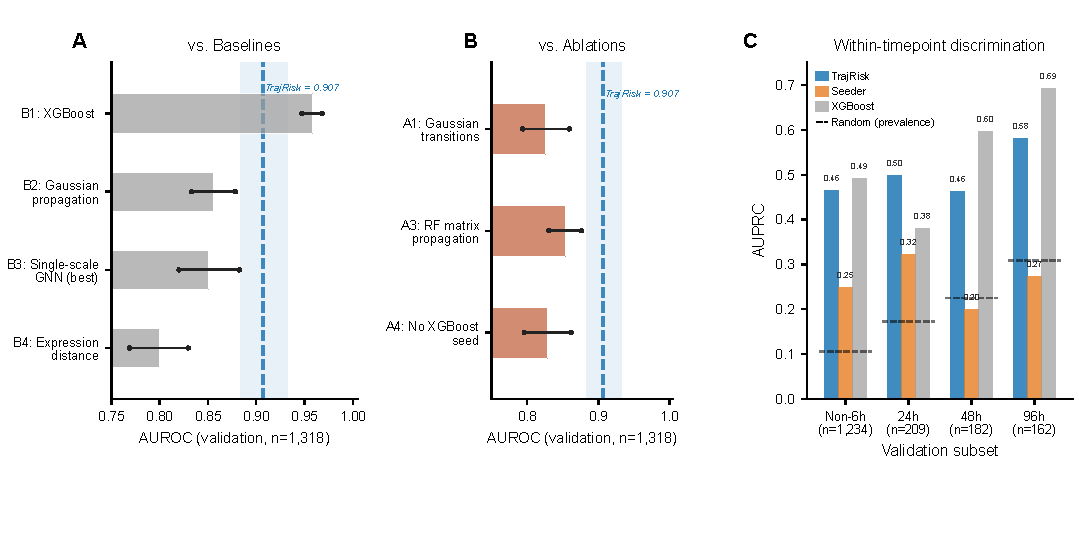
\includegraphics[width=\textwidth,trim={0.000bp 0.000bp 0.000bp 0.000bp},clip]{figures/figure_4.pdf}
\caption{\textbf{\FigFourTitle{}} \textbf{(A)} \FigFourA{} \textbf{(B)} \FigFourB{} \textbf{(C)} \FigFourC{} \FigFourNotes{}}
\label{fig:4}
\end{figure*}

\subsection*{External mouse transfer is cohort-dependent}

We evaluated three external mouse cohorts using frozen Walesky-trained models (\FigRef{5}{A}; \TableRef{S3A}). In Ben-Moshe hepatocytes (n = 2,770), APAP-versus-control AUROC was 0.7197 for Reference-KNN and 0.8069 for \SelfOnly{} TrajRisk, compared with 0.8541 for the seed and 0.8544 for B1. In the Umbaugh 48/72~h cohort (n = 5,306), the corresponding AUROCs were 0.7939, 0.8958, 0.9330, and 0.9423. Both TrajRisk variants therefore underperformed expression-only comparators on treatment discrimination in these later cohorts. Treatment status is a different endpoint from the normalized reference pseudotime used for TrajRisk training; this distinction does not by itself establish that lower transferred scores accurately identify recovery.

At Umbaugh 2~h, a sampling time absent from supervised model training (n = 21,409), Reference-KNN AUROC was 0.6524, compared with 0.6087 for \SelfOnly{}, 0.6465 for the seed, and 0.6422 for B1 (\FigRef{5}{B}; \TableRef{S3A}). Reference-KNN thus showed a small observed advantage over the expression-only comparators at early injury, with no reported pairwise significance test. External cohorts were included in the unsupervised scVI integration, so frozen-model transfer here does not represent evaluation of an entirely unseen expression distribution.

In all 5,306 Umbaugh 48/72~h hepatocytes, \SelfOnly{} scores correlated positively with \textit{Cdkn1a} expression (Spearman \ensuremath{\rho} = 0.382; p = 3.84\ensuremath{\times}10\textsuperscript{-184}; \FigRef{5}{C}; \TableRef{S3B}). Reference-KNN had \ensuremath{\rho} = 0.313, whereas the seed and B1 had stronger correlations (0.418 and 0.404). The association connects the transferred score to a p21-associated transcriptional program but does not demonstrate added information over expression-only comparators or a causal mechanism; \textit{Cdkn1a} transcript detection does not directly measure p21 protein.

\begin{figure*}[!tp]
\centering
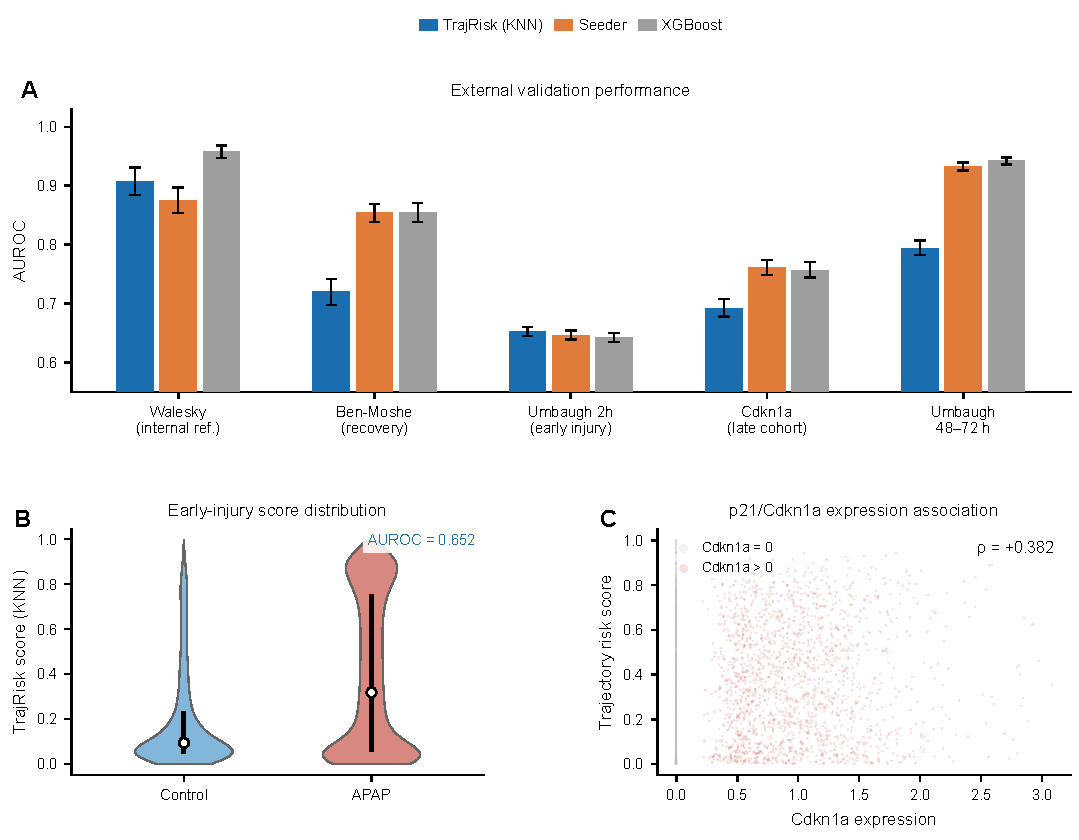
\includegraphics[width=\textwidth,trim={0.000bp 0.000bp 0.000bp 0.000bp},clip]{figures/figure_5.pdf}
\caption{\textbf{\FigFiveTitle{}} \textbf{(A)} \FigFiveA{} \textbf{(B)} \FigFiveB{} \textbf{(C)} \FigFiveC{} \FigFiveNotes{}}
\label{fig:5}
\end{figure*}

\subsection*{TrajRisk transfers the mouse trajectory-state score to human APAP-ALF donors}

Cross-species scVI integration of Walesky mouse hepatocytes and Matchett human hepatocyte nuclei used 13,122 shared mouse--human gene-symbol pairs retained by the uniqueness and expression-axis filters (\FigRef{6}{A}; \TableRef{S4A}). Quality-control characteristics of the 49,984 Matchett human hepatocyte nuclei are summarized in \FigRef{S1}{D}. Both species and condition ASW rounded to 0.0347, consistent with mixing in the joint latent space; the shared cross-species scVI space visualized by species and biological condition is shown in \FigRefs{S3}{A and S3B}. Donor-level \SelfOnly{} TrajRisk scores were higher in APAP-ALF donors (n = 10) than healthy donors (n = 9) (mean 0.2051 vs. 0.1088; Mann-Whitney p = 6.4\ensuremath{\times}10\textsuperscript{-3}; donor-level AUROC = 0.844; \FigRef{6}{B}; \TableRef{S4B}; \DataRef{S3}). Nucleus-level primary \SelfOnly{} scores across the same cross-species latent coordinates are shown in \FigRef{S3}{C}.

A Reference-KNN sensitivity analysis gave consistent results (p = 8.0\ensuremath{\times}10\textsuperscript{-3}; AUROC = 0.833; \TableRef{S4B}; \DataRef{S3}). The temporal composition of the 15 nearest Walesky reference neighbors used in this sensitivity analysis is summarized by human condition in \FigRef{S3}{D}; this panel is a reference-projection diagnostic rather than human trajectory inference. The primary \SelfOnly{} association remained significant after exclusion of low-nucleus-count donors (p = 2.5\ensuremath{\times}10\textsuperscript{-2}; AUROC = 0.815; \FigRef{6}{C}; \TableRef{S4B}; \DataRef{S4}).

The raw orthologous risk signature, defined by genes positively correlated with mouse pseudotime (\DataRef{S1}), had lower donor means in APAP-ALF than in healthy tissue (0.3585 versus 0.4380) and AUROC 0.056 in its prespecified direction (\TableRef{S4B}). Subtracting the 50-gene recovery signature gave a net-signature AUROC of 0.656, but the directional donor comparison remained non-significant (p = 0.135). The net signature therefore did not independently validate case--control discrimination. Reference-KNN TrajRisk and net-signature donor scores were correlated (Spearman \ensuremath{\rho} = 0.833; p = 9.4\ensuremath{\times}10\textsuperscript{-6}; \FigRef{6}{D}; \TableRef{S4C}; \DataRef{S3}). Because both use the same expression data and the cohort contains only 19 donors, this association describes concordant ordering rather than independent replication.

Human differential-expression overlap with mouse bottleneck-associated genes is reported below alongside the bottleneck analysis (\FigRef{6}{E}).

\begin{figure*}[!tp]
\centering
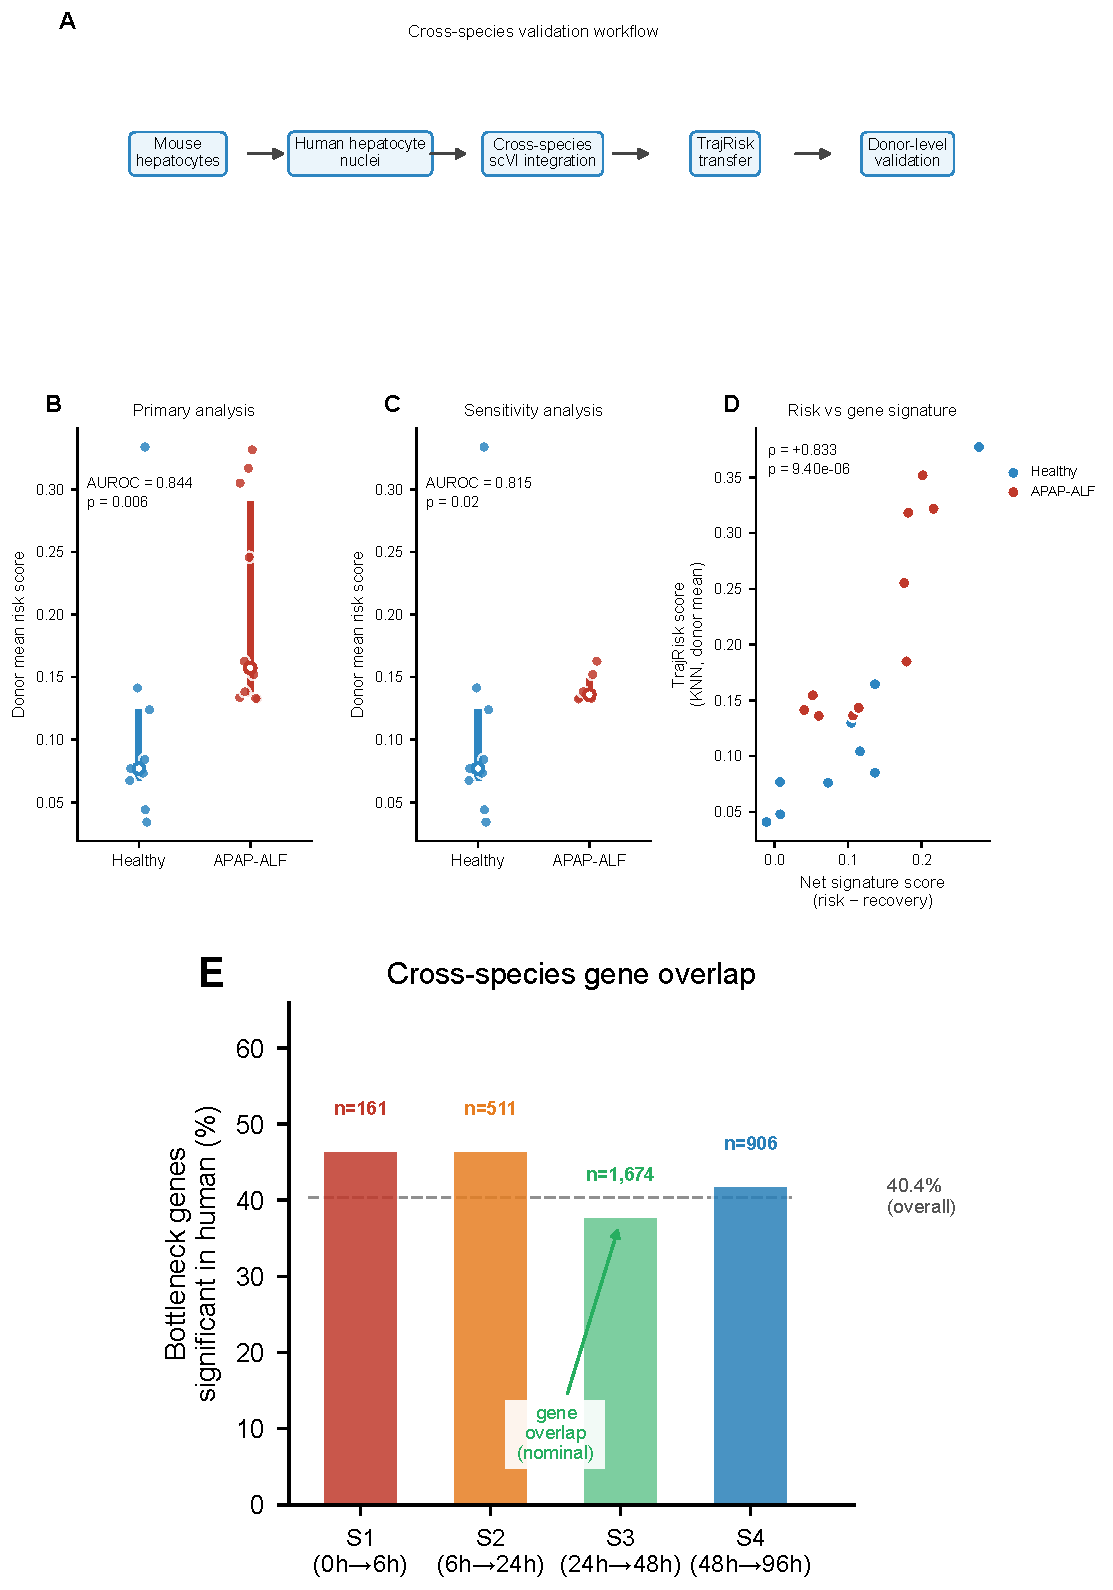
\includegraphics[width=\textwidth,trim={0.000bp 670.000bp 0.000bp 0.000bp},clip]{figures/figure_6.pdf}
\par\vspace{7pt}
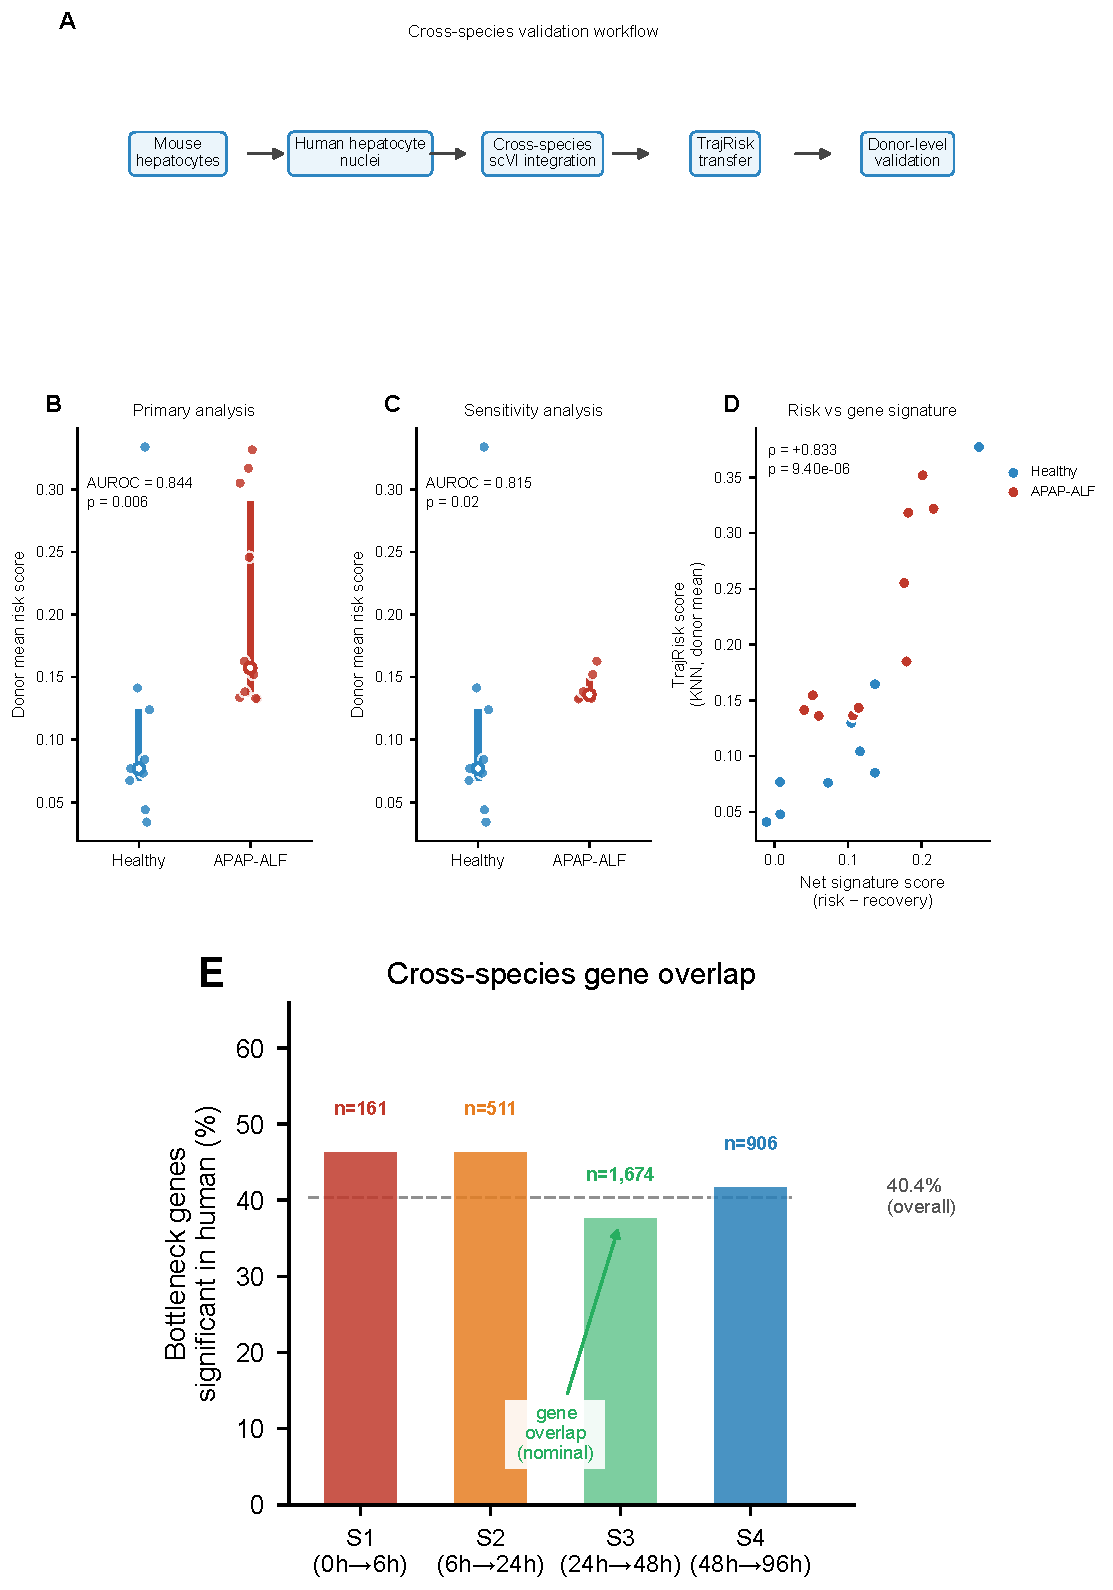
\includegraphics[width=\textwidth,trim={0.000bp 321.000bp 0.000bp 186.000bp},clip]{figures/figure_6.pdf}
\caption{\textbf{\FigSixTitle{}} \textbf{(A)} \FigSixA{} \textbf{(B)} \FigSixB{} \textbf{(C)} \FigSixC{} \textbf{(D)} \FigSixD{} \FigSixNotes{}}
\label{fig:6}
\end{figure*}
\begin{figure*}[!tp]
\centering
\ContinuedFloat
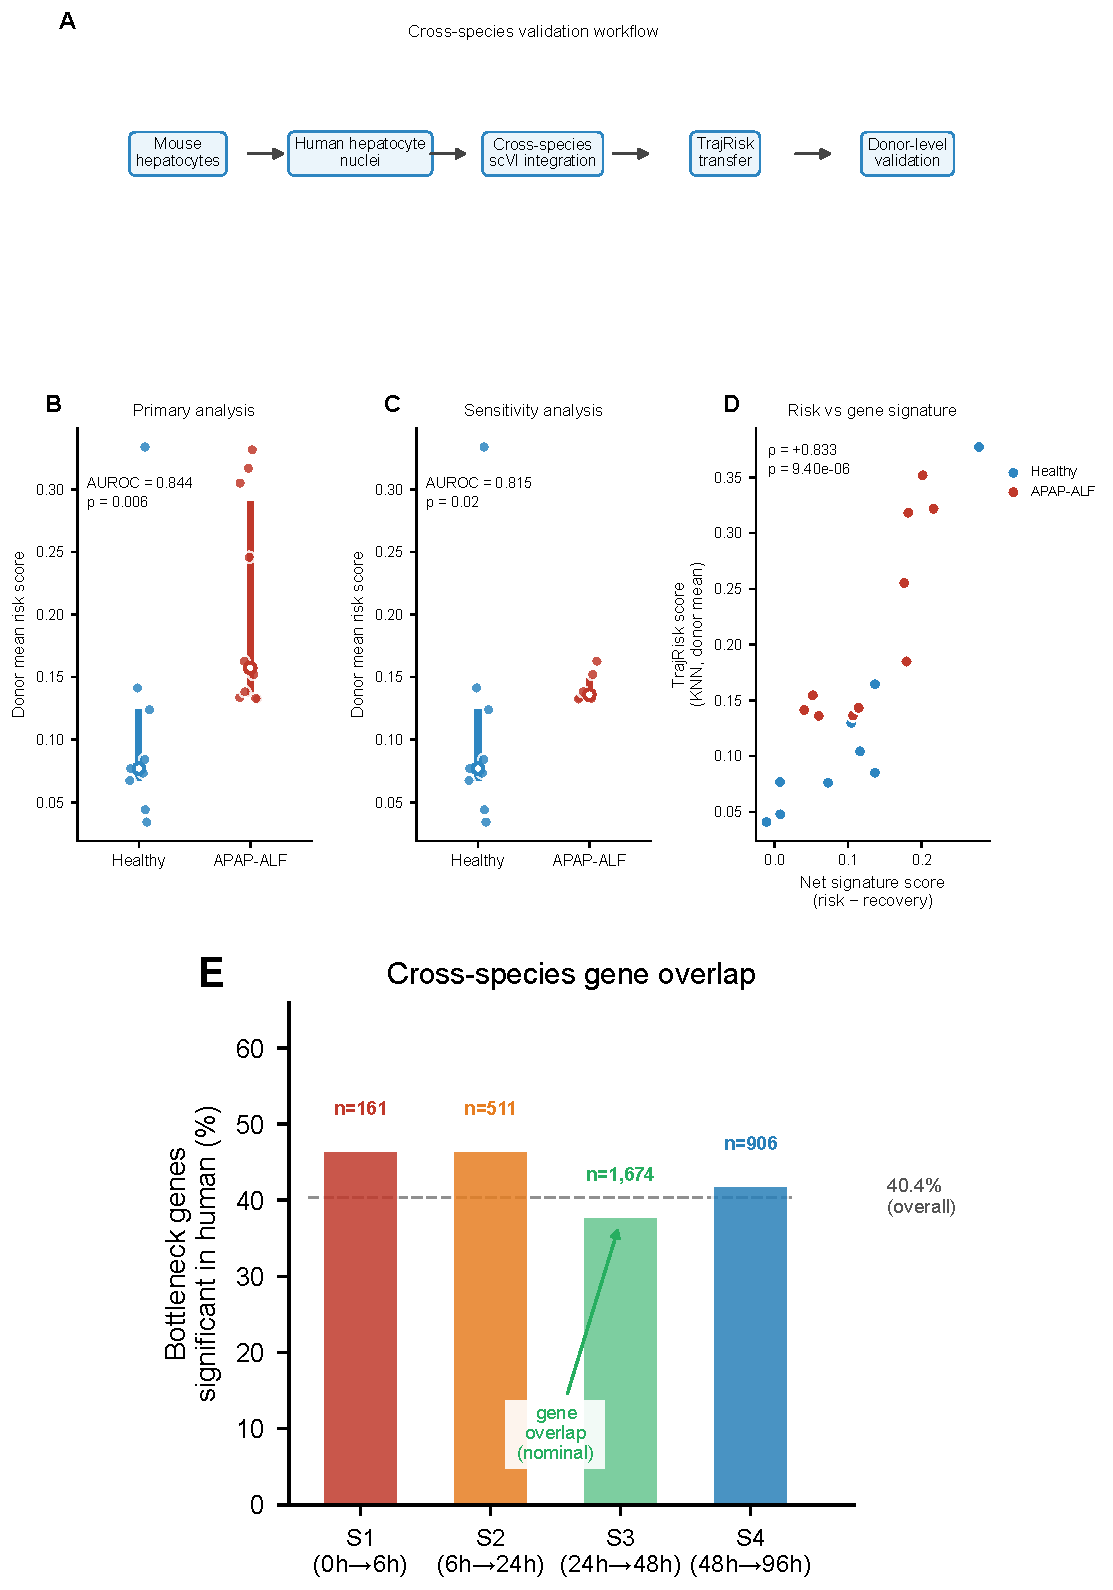
\includegraphics[width=0.79\textwidth,trim={74.000bp 0.000bp 21.000bp 447.000bp},clip]{figures/figure_6.pdf}
\caption{\textbf{\FigSixTitle{} (continued)} \textbf{(E)} \FigSixE{}}
\end{figure*}

\subsection*{Spatial localization of the orthologous risk signature varies across datasets}

We next evaluated whether the orthologous TrajRisk risk signature localized to spatial regions associated with APAP injury using two independent Visium studies (\FigRef{S4}{}). In the Ben-Moshe spatial dataset, fibrogenic spots marking the pericentral necrotic boundary were significantly enriched for the TrajRisk signature (pooled one-sided Mann--Whitney p < 10\textsuperscript{-300}); enrichment remained significant at 24~h (p = 1.55\ensuremath{\times}10\textsuperscript{-48}), 48~h (p = 9.37\ensuremath{\times}10\textsuperscript{-300}), and 72~h (p = 1.19\ensuremath{\times}10\textsuperscript{-301}), consistent with localization to regions of active injury (\FigRef{S4}{A}; \TableRef{S5A}). These exploratory tests pool spots and do not estimate significance across independent biological replicates.

By contrast, the TrajRisk \textbf{risk signature} was not enriched in anatomically defined pericentral regions of either Matchett spatial dataset. In mouse Visium sections, risk-signature scores were similar between pericentral and periportal spots (one-sided Mann--Whitney p = 0.087; \FigRef{S4}{B}; \TableRef{S5B}), whereas in human sections the pericentral-greater-than-periportal hypothesis was not supported (p = 1.000; \FigRef{S4}{D}; \TableRef{S5C}). Risk-signature scores were negatively correlated with \textit{Cyp2e1/CYP2E1} expression in both mouse (\ensuremath{\rho} = \ensuremath{-}0.427) and human (\ensuremath{\rho} = \ensuremath{-}0.168) tissue (\TableRefs{S5B}{S5C}). In contrast, after excluding \textit{Cyp2e1/CYP2E1} itself from the recovery signature to avoid circularity with zone definition, recovery-signature scores were significantly lower in pericentral than periportal regions in both mouse (p = 1.31\ensuremath{\times}10\textsuperscript{-57}; \FigRef{S4}{C}; \TableRef{S5B}) and human (p = 2.96\ensuremath{\times}10\textsuperscript{-153}; \FigRef{S4}{E}; \TableRef{S5C}) datasets. APAP-ALF human sections nevertheless showed descriptively higher mean risk-signature scores than healthy sections across pericentral, midlobular, and periportal zones (\FigRef{S4}{F}; \TableRef{S5D}; \DataRef{S5}); no zone-level case-control significance test was performed because spots within a section are not independent biological replicates.

\subsection*{Bottleneck analysis identifies scale-specific programs and a candidate recovery gateway}

Risk flux analysis across 421,477 graph edges (\hyperref[sec:methods]{Methods}) showed that Scale 2 (Peak Injury, 6~h \ensuremath{\rightarrow} 24~h) carried the largest total flux, with 98.5\% of its edges showing negative amplification as TrajRisk scores decreased from the peak. In contrast, Scale 1 (Acute Stress, 0~h \ensuremath{\rightarrow} 6~h) edges showed uniformly positive amplification. The heavy-tailed risk-flux distributions across all four scales are shown in \FigRef{7}{A} (\TableRef{S6A}). Scale 1 ablation produced the largest total change in TrajRisk scores, showing the greatest sensitivity of the frozen model to removal of that scale (\FigRef{7}{D}; \TableRef{S6B}).

Scale 3 (Fate Decision, 24~h \ensuremath{\rightarrow} 48~h) showed the highest flux concentration, with 9.8\% of total scale flux carried by the top 1\% of edges (\TableRef{S6A}). The pseudotime distribution of top-flux source cells was bimodal at Scale 3, spanning both recovery-proximal and persistent-compensation 24~h states (\FigRef{7}{B}). The 43 unique 24~h source cells feeding these high-flux edges were enriched for elevated scores and pseudotime within the 24~h population: all 43 were in the top TrajRisk-score quartile among 24~h cells, and 76.7\% were high-pseudotime. By contrast, only 18.9\% of the 380 unique 48~h target cells were high-pseudotime, below the 25.1\% expected background proportion (\FigRef{7}{C}; \TableRefs{S6C}{S6D}). The source-cell enrichment was robust to the bottleneck definition: across top 0.5\%, 1\%, 2\%, 5\%, and 10\% Scale 3 flux thresholds, the fraction of high-pseudotime source cells remained above the 25.0\% background among all 24~h cells (\FigRef{S5}{A}; \TableRef{S6E}). These connections motivate a candidate resolution-gateway hypothesis linking compensation-associated 24~h states to recovery-proximal 48~h states. Flux contains the source score by definition, so enrichment of high-score sources is partly built into the selection. Neither lineage transitions nor a causal role in recovery are established by this model-derived analysis. In a complementary perturbation analysis, mean absolute 48~h score changes remained small across source-cell pseudotime quartiles (0.0015--0.0018), whereas the Q4 high-pseudotime group produced the largest maximum single-cell change (0.0979); all 96~h mean and maximum effects were zero (\FigRef{S5}{B}; \TableRef{S6F}).

Pathway analysis showed scale-specific programs: Scale 1 bottleneck targets were enriched for oxidative phosphorylation; Scale 2 targets showed lower expression of CYP-associated metabolic programs; Scale 3 targets showed downregulation of ribosome biogenesis, mitochondrial translation, and immediate-early stress-response programs; and Scale 4 targets showed enrichment of periportal-associated programs (\FigRef{7}{F}). Scale 3 bottleneck edges also showed significantly larger embedding shifts than background edges (p < 10\textsuperscript{-172}; \FigRef{7}{E}; \TableRef{S6G}), consistent with Scale 3 being a representational as well as a flux bottleneck.

We separately assessed human differential-expression overlap with mouse bottleneck-associated programs. Among 2,549 tested mouse-gene mappings, 1,036 (40.6\%) met the nominal human differential-expression criterion in APAP-ALF versus healthy donors (p \ensuremath{\leq} 0.05; \DataRef{S2}). These records correspond to 1,023 significant human genes among 2,534 distinct human genes tested (40.4\%). The corresponding distinct-human-gene overlap was 46.6\%, 46.6\%, 37.8\%, and 41.9\% for Scales 1--4, respectively (\FigRef{6}{E}). The criterion requires nominal significance in human donors, but not agreement in fold-change direction between species. These overlaps are exploratory, unadjusted for multiple testing, and not benchmarked against a matched gene background; cross-sectional human sampling also does not reproduce the temporally defined mouse transitions.

\begin{figure*}[!tp]
\centering
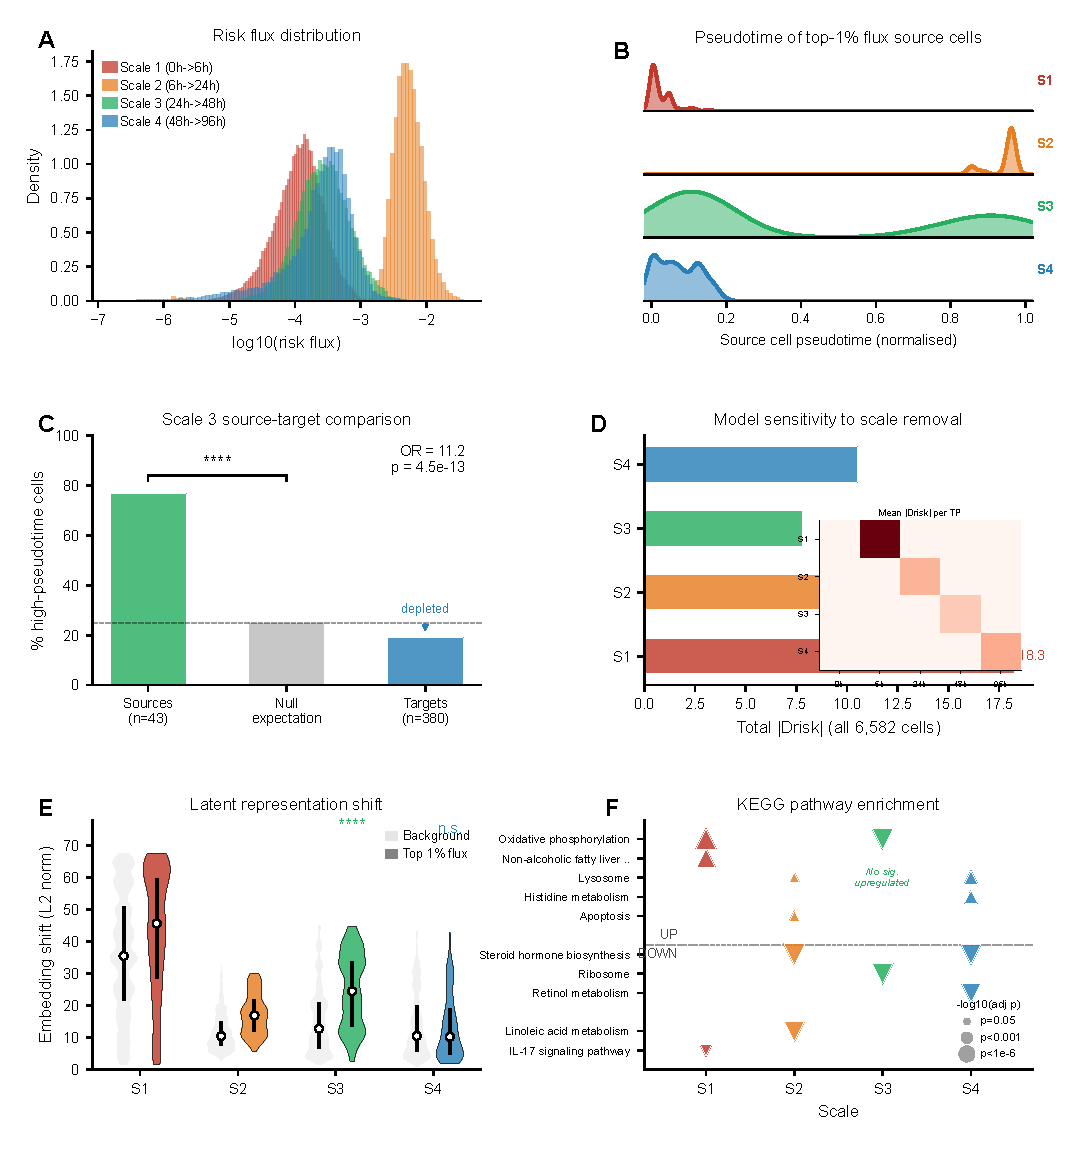
\includegraphics[width=\textwidth,trim={0.000bp 197.000bp 0.000bp 0.000bp},clip]{figures/figure_7.pdf}
\caption{\textbf{\FigSevenTitle{}} \textbf{(A)} \FigSevenA{} \textbf{(B)} \FigSevenB{} \textbf{(C)} \FigSevenC{} \textbf{(D)} \FigSevenD{} \FigSevenNotes{}}
\label{fig:7}
\end{figure*}
\begin{figure*}[!tp]
\centering
\ContinuedFloat
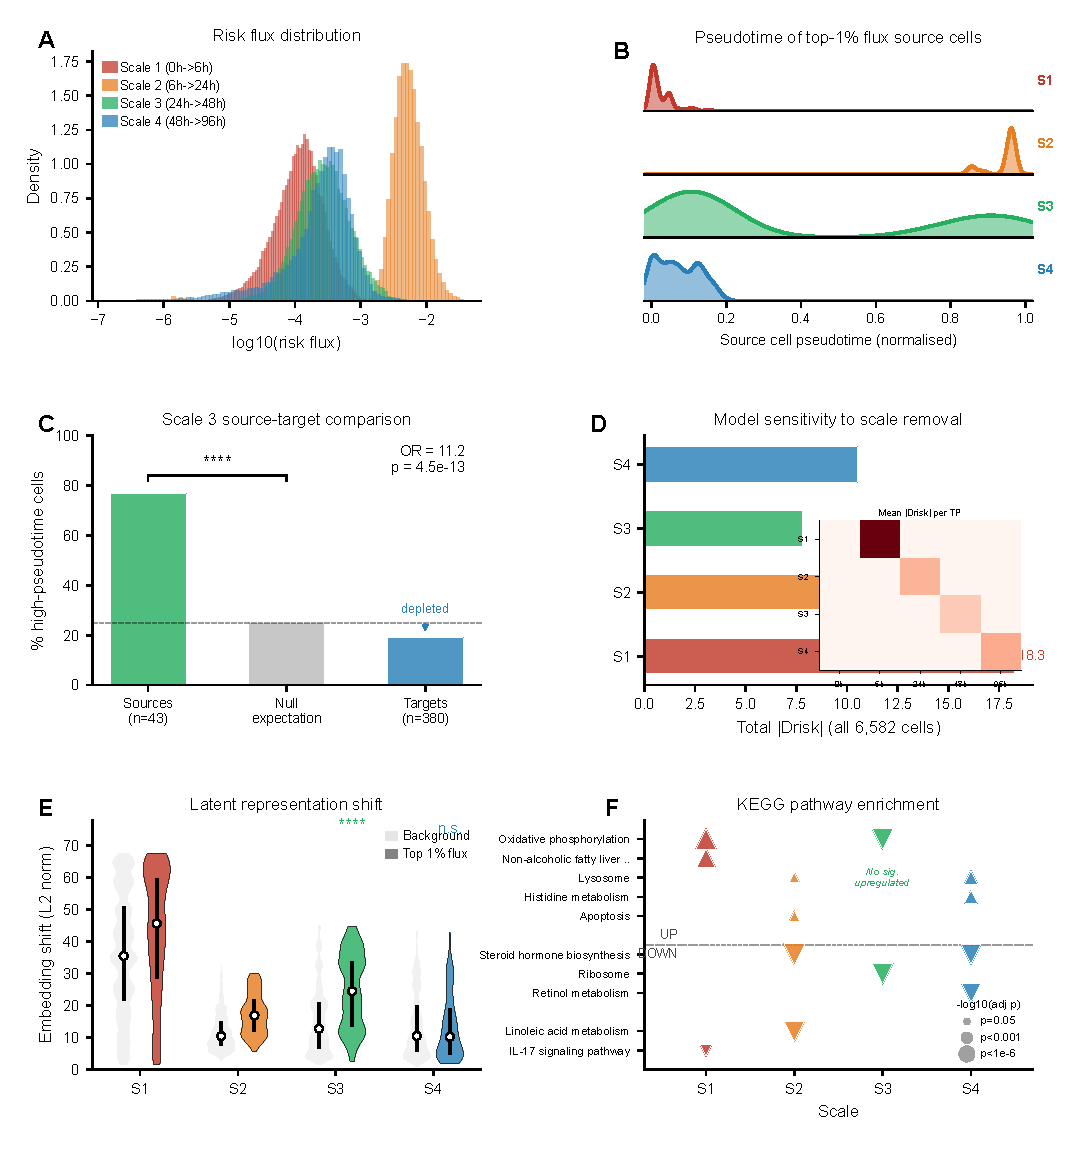
\includegraphics[width=\textwidth,trim={0.000bp 0.000bp 0.000bp 372.000bp},clip]{figures/figure_7.pdf}
\caption{\textbf{\FigSevenTitle{} (continued)} \textbf{(E)} \FigSevenE{} \textbf{(F)} \FigSevenF{}}
\end{figure*}

